% !TEX root = ../22830110_dissertation.tex

\chapter{Testing and Evaluation Strategy}
\label{chap:testing_evaluation}

\section{Quantitative Evaluation Framework}
The quantitative assessment of the system focuses on strict numerical fidelity, completeness, grounding, and efficiency. The evaluation strategy follows the comparative framework established in Chapter \ref{chap:methodology}: the live benchmark compares four callable GPT-4.1 fine-tuned deployments with a GPT-5.4 prompt-engineering baseline deployed through Azure AI Foundry. The GPT-5.4 deployment is accessed through the Azure OpenAI-compatible endpoint, with all credentials supplied through environment variables rather than being embedded in source code.

The prompt-engineering baseline is tested under three conditions:
\begin{itemize}
    \item \textbf{Zero-Shot Prompting:} The model receives only the accountant role instruction and the target Xero-derived context.
    \item \textbf{Single-Shot Prompting:} The model receives one complete exemplar review note before the target validation case.
    \item \textbf{Few-Shot Prompting:} The model receives three exemplars representing different review-note structures before the target validation case.
\end{itemize}

The live comparative evaluation harness is implemented in \path{experiments/benchmark_dissertation_methods.py}, with prompt-construction helpers in \path{experiments/prompt_engineering_gpt54.py}. It loads the validation JSONL file, constructs the appropriate prompt for each condition, calls the \texttt{gpt-5.4} deployment and the callable GPT-4.1 fine-tuned deployments, and records the generated text, token usage, latency, strategy, and matching gold response to CSV. These outputs are then scored using the existing scoring framework against the following criteria:
\begin{itemize}
    \item \textbf{Numeric Fidelity:} Whether monetary values, tax liabilities, and percentage movements match the structured Xero context and gold note.
    \item \textbf{Completeness:} Whether mandatory sections such as Corporation Tax, Balance Sheet, Directors' Loan Account, and recommendations are present where applicable.
    \item \textbf{Grounding and Provenance:} Whether generated statements are supportable by ledger codes, trial balance lines, or transaction context.
    \item \textbf{Narrative Constraints:} Whether the output follows the PHM ``You'' style, statutory sequencing, and concise working-paper structure.
    \item \textbf{Edit Distance and Latency:} How much human editing is implied relative to the gold response, and how long each generation takes.
\end{itemize}

\begin{figure}[H]
    \centering
    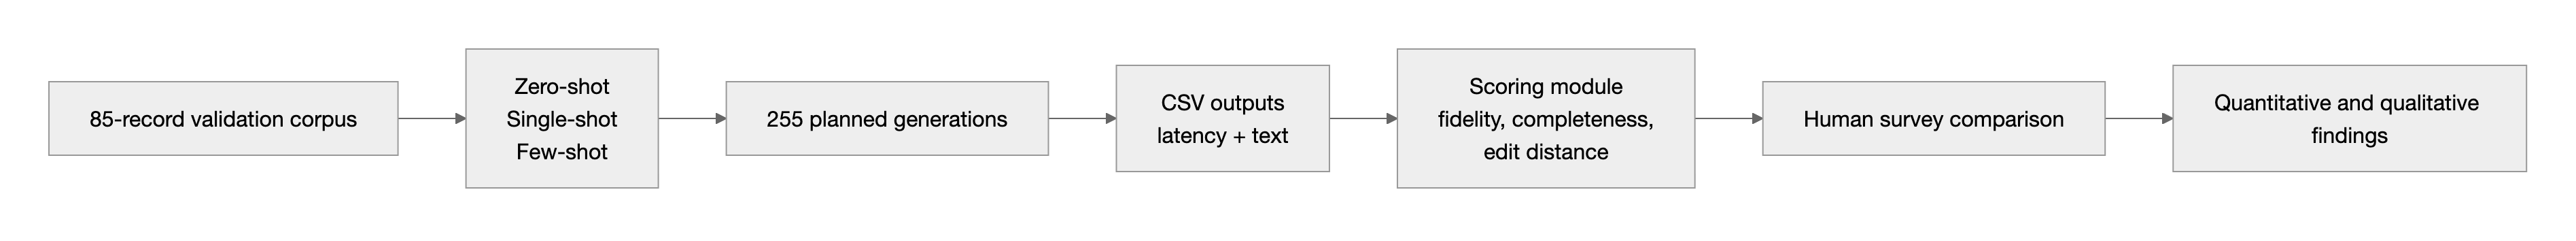
\includegraphics[width=0.9\textwidth]{figures/evaluation_workflow}
    \caption{End-to-End Evaluation Workflow for Prompt Engineering and Human Review}
    \label{fig:evaluation_workflow}
\end{figure}

Figure \ref{fig:evaluation_workflow} shows the evaluation flow used in practice: the validation corpus is passed through the three prompt conditions, written to CSV, scored, and then read alongside the survey results.

The fine-tuned arm of the comparison was designed around three recipes rather than a single monolithic model. FT-A preserves the raw working-paper style most directly. FT-B uses scrubbed notes to reduce noisy narrative habits. FT-C adds deterministic rule cues from the data pipeline so that recurring subscriptions, material movements, and mandatory comment accounts are made more legible before generation begins. In the live Foundry project, however, four callable GPT-4.1 fine-tuned deployments were available at benchmark time. All four were therefore kept in the final comparison to avoid cherry-picking.

\section{Validation Corpus}
The prompt-engineering test set uses \texttt{exceptional\_validation\_data.jsonl}, containing 85 accountant-authored validation examples. Each record contains a system prompt, Xero-derived trial balance context, and the corresponding accountant-written target review note. The corpus is intentionally demanding: the average record contains approximately 161 monetary mentions and 7,500 characters of combined prompt and target text. This makes it suitable for testing whether GPT-5.4 can preserve numeric precision over long, dense accounting contexts.

\begin{figure}[H]
    \centering
    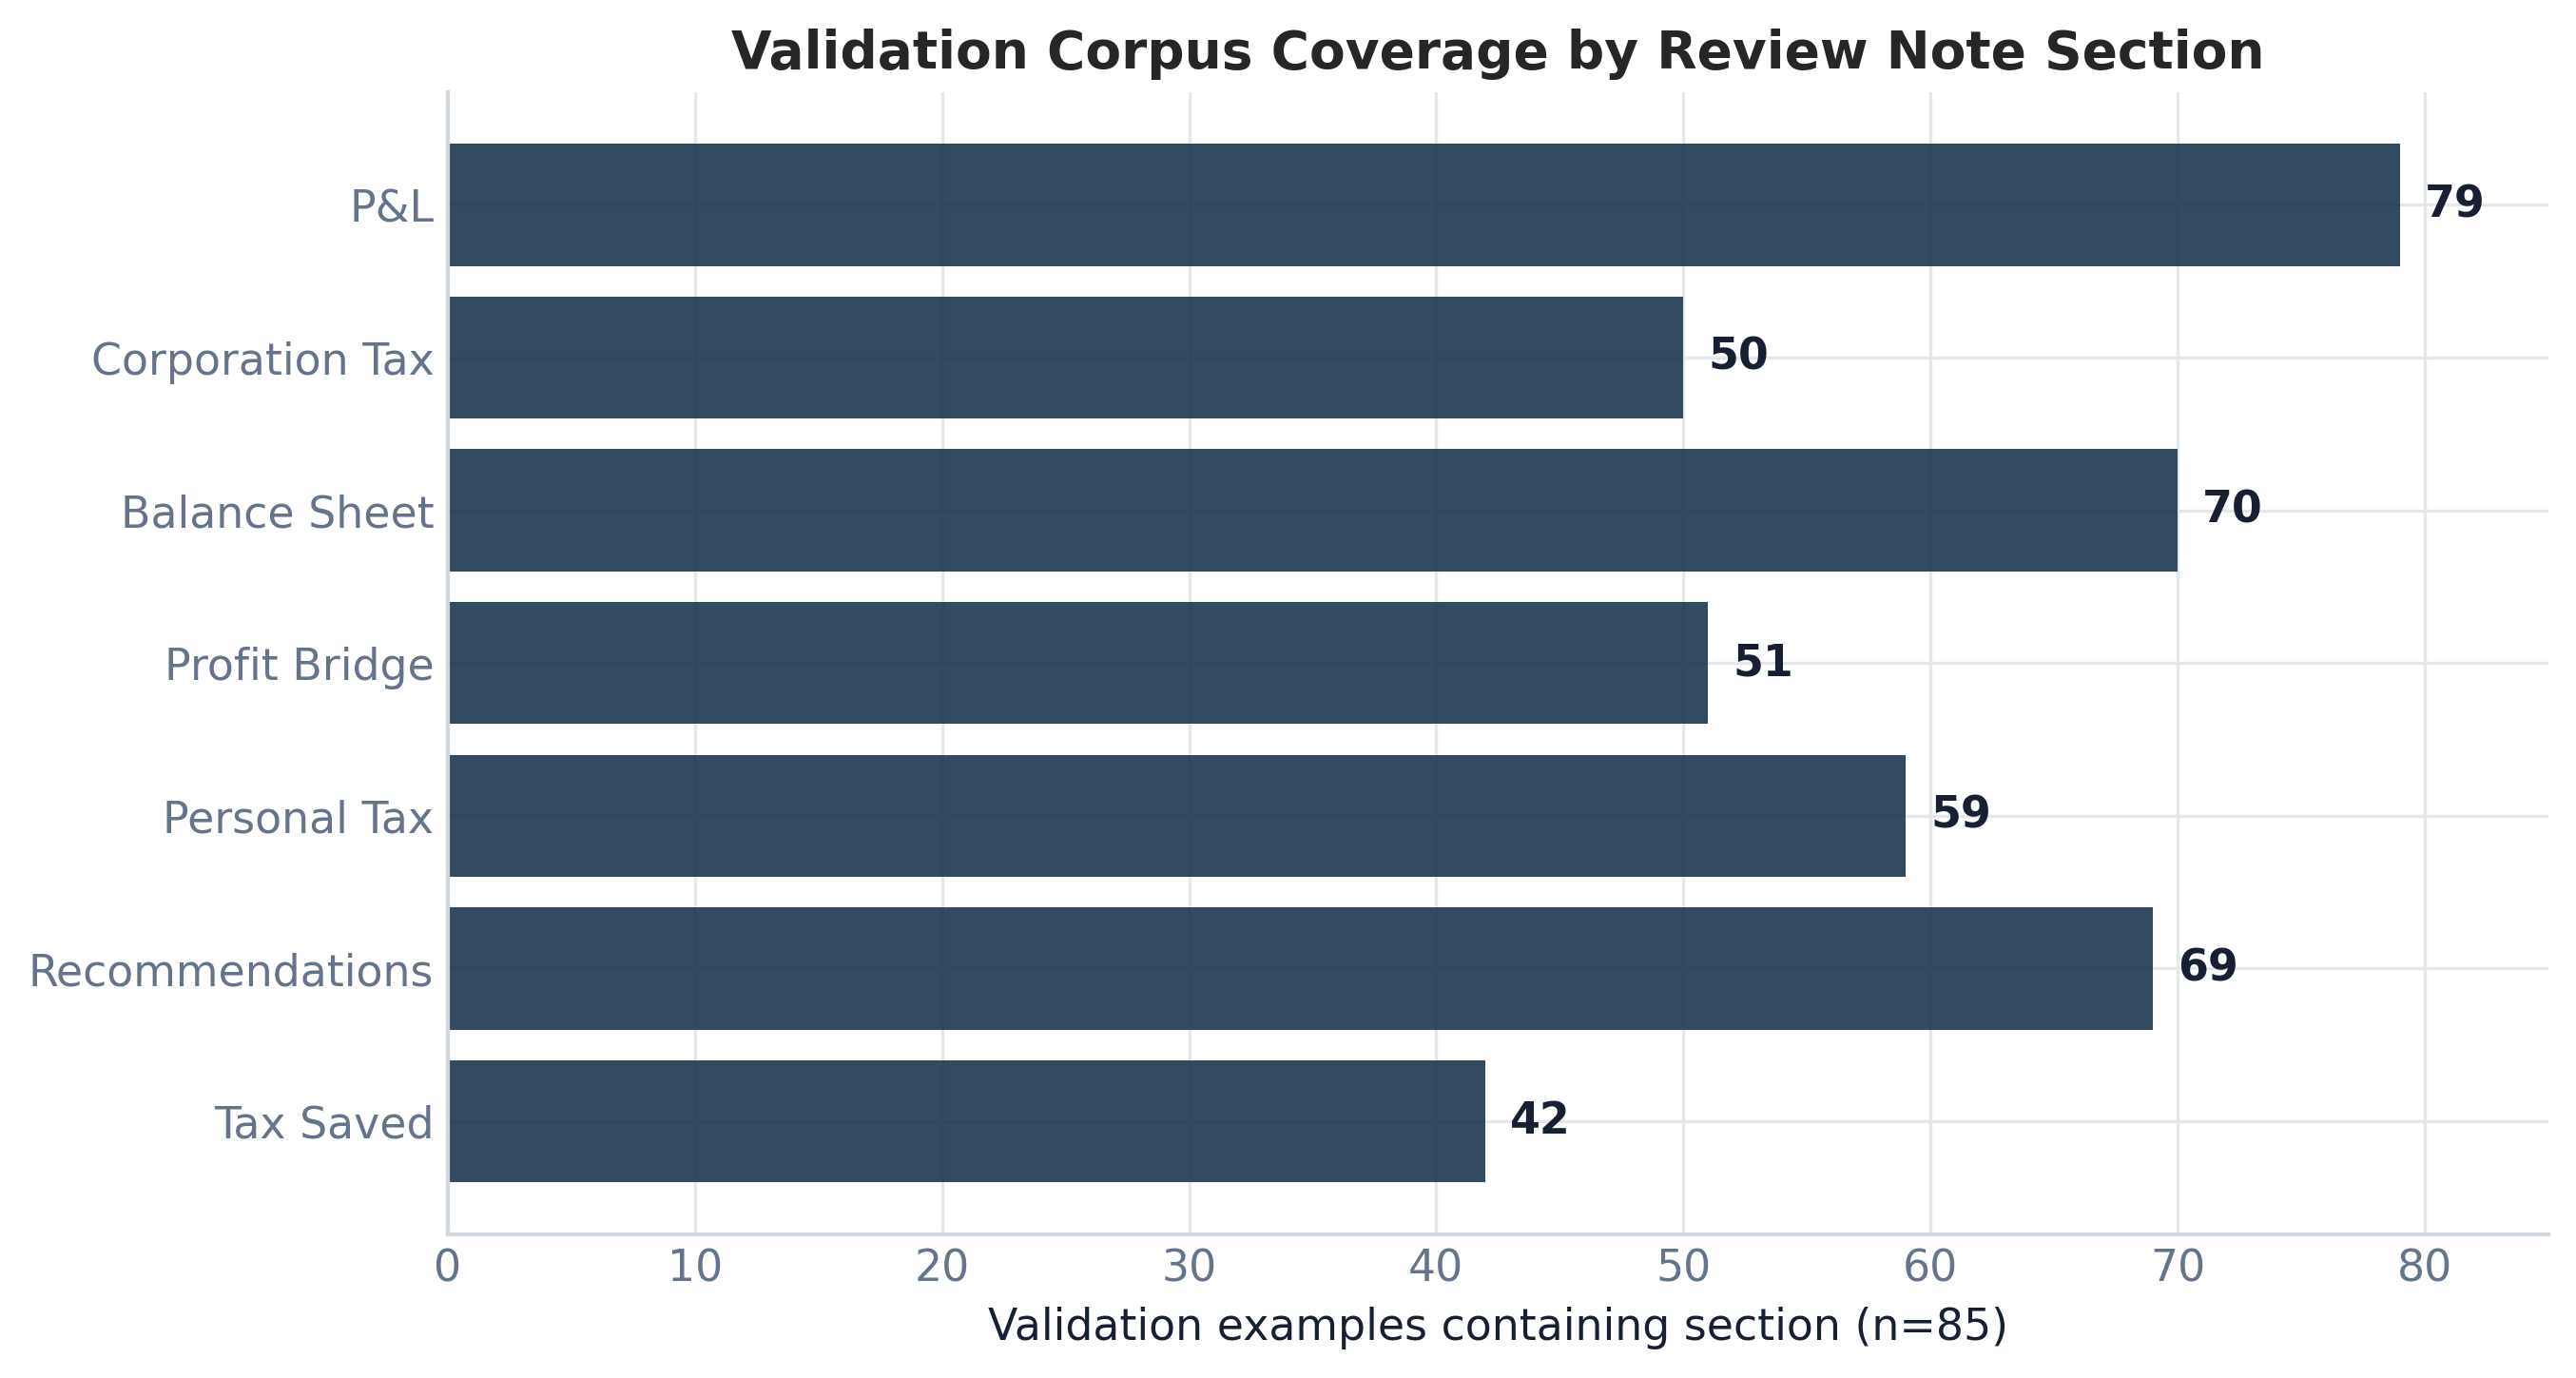
\includegraphics[width=0.86\textwidth]{figures/validation_section_coverage}
    \caption{Coverage of Key Review Note Sections in the Validation Corpus}
    \label{fig:validation_section_coverage}
\end{figure}

Figure \ref{fig:validation_section_coverage} shows that the validation corpus covers the major note families required for the application. Profit and loss commentary is the most common section, appearing in 79 of 85 records, followed by Balance Sheet commentary in 70 records and recommendations in 69 records. Corporation Tax, personal tax, profit-bridge commentary, and tax-saved explanations are also represented, ensuring that the prompt-engineering comparison tests more than simple profit-and-loss summarisation.

The corpus does not consist only of easy examples where the correct answer is a paraphrase of a trial balance. It also includes cases where the accountant's note is a warning, a query, or a request for missing evidence. One real validation record centres on unresolved share issue paperwork; another includes GDPR-related compliance spend within staff-training commentary; another discusses an overdrawn director's loan account and the need to monitor post-year-end clearance. These cases matter because they test whether the system can distinguish between explanation and unresolved review points.

\begin{figure}[H]
    \centering
    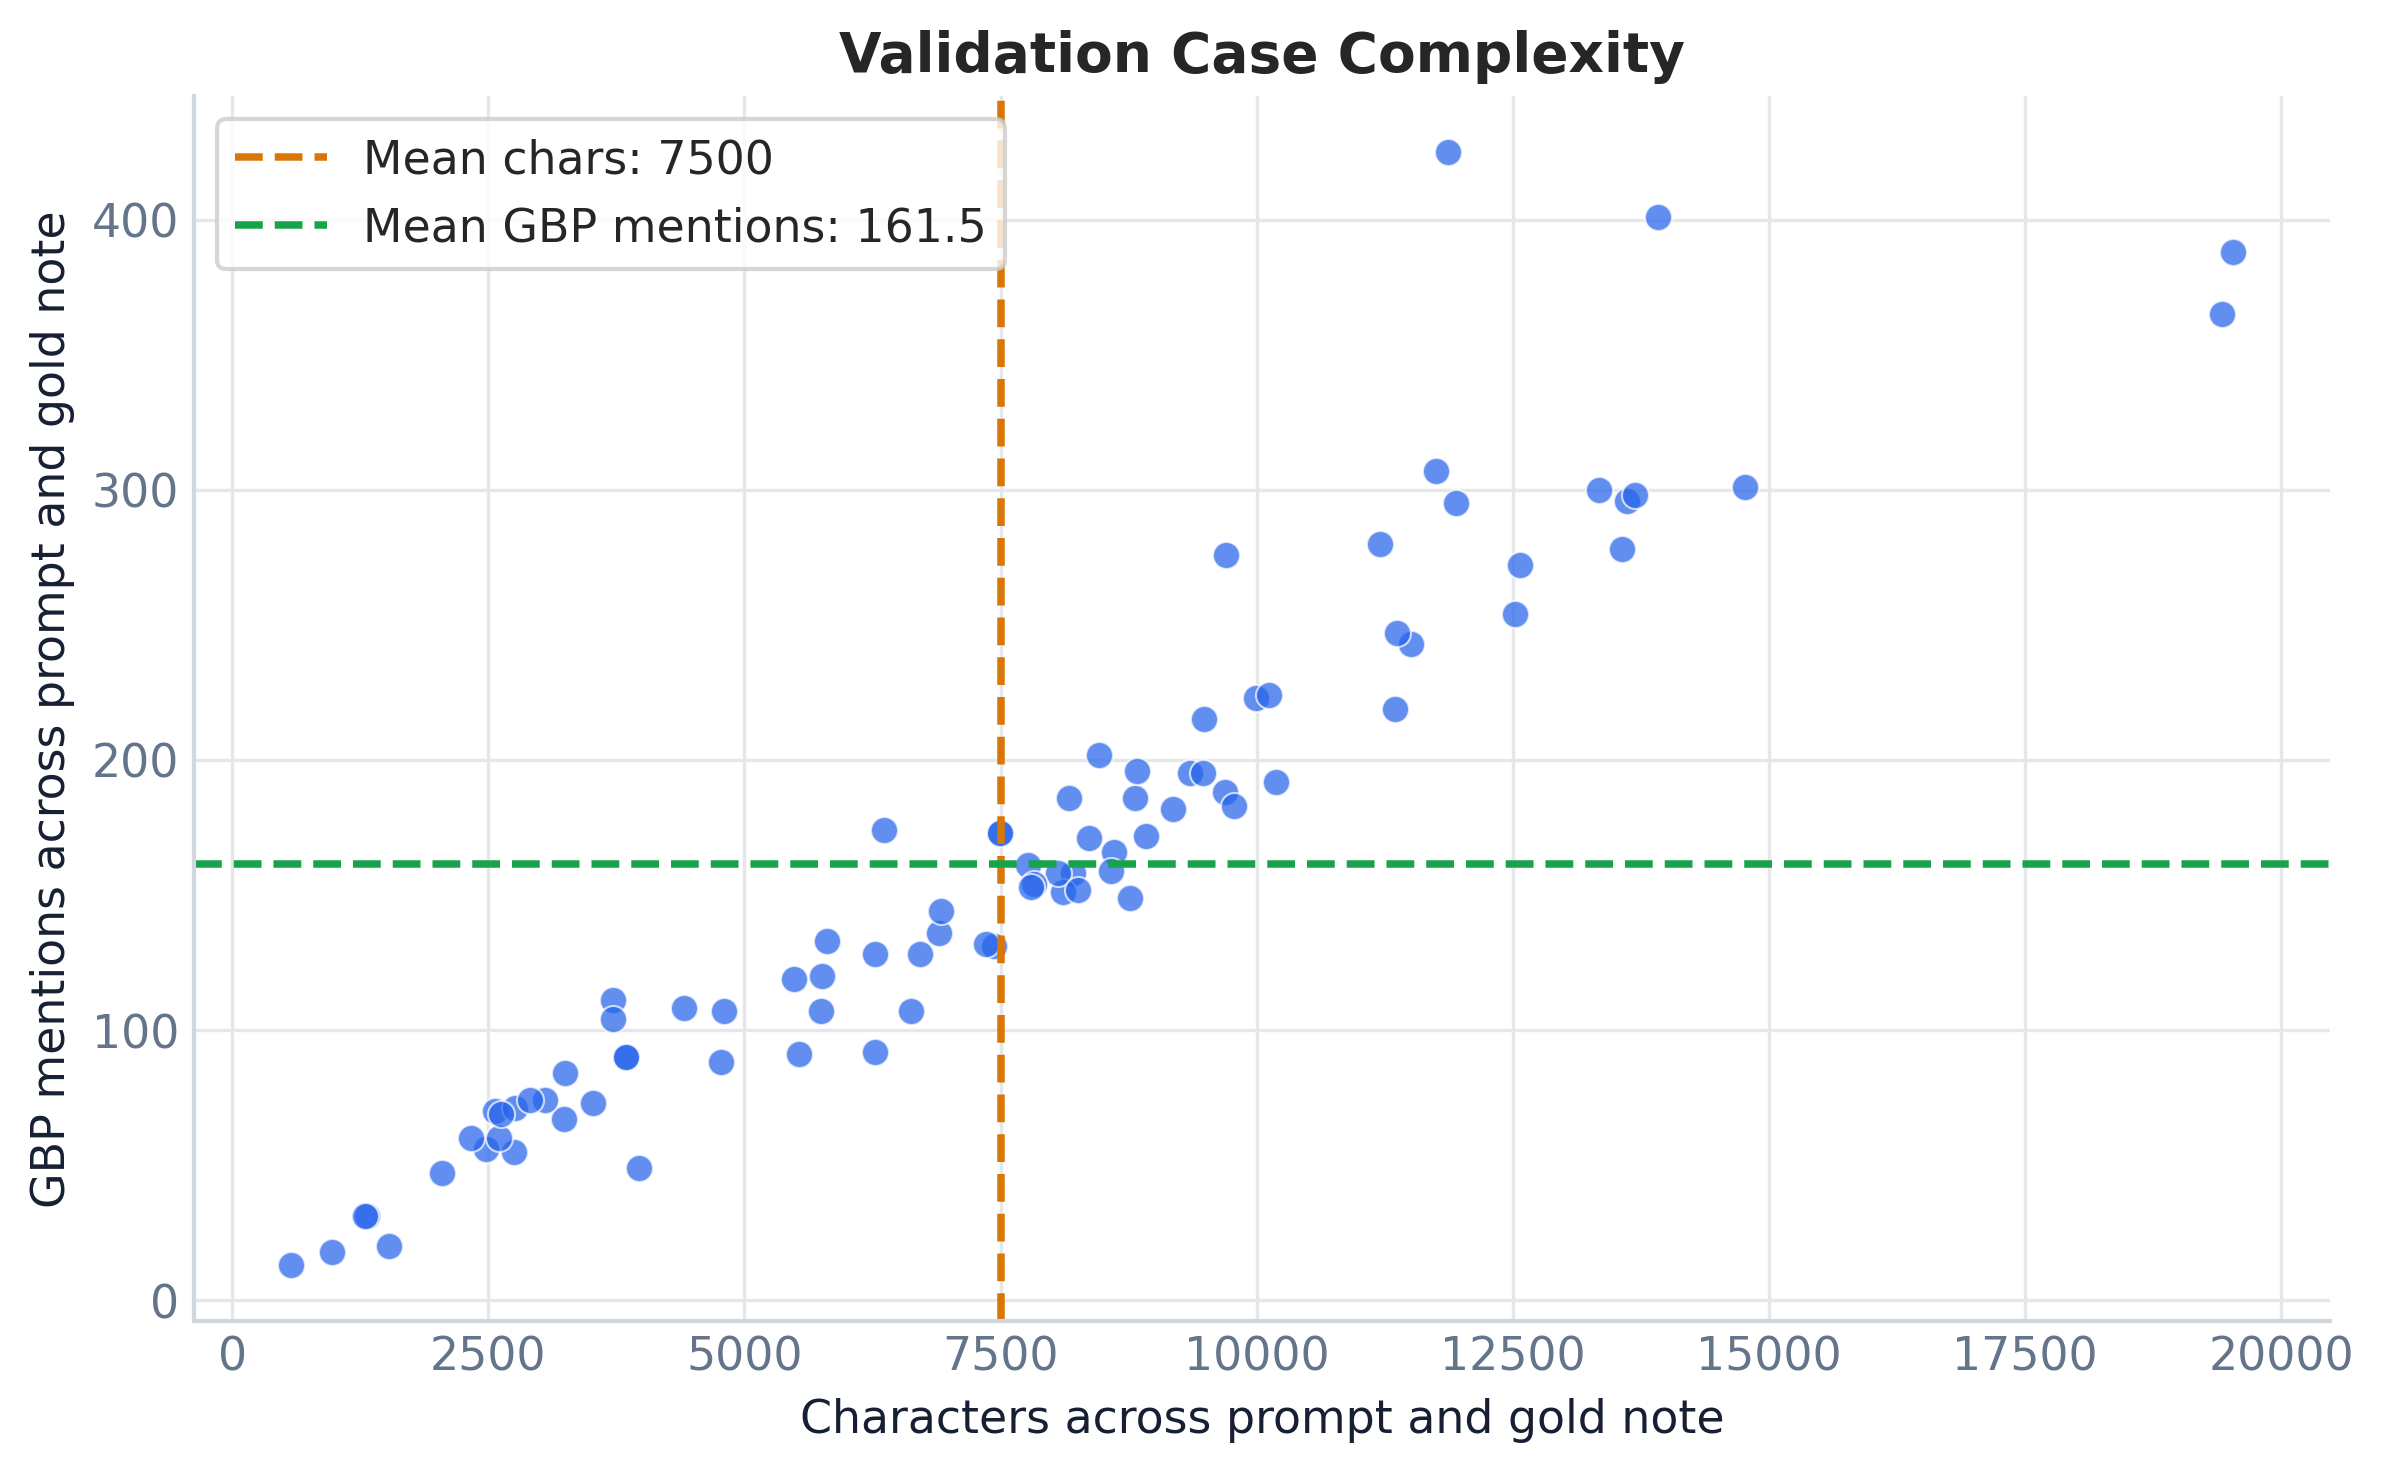
\includegraphics[width=0.8\textwidth]{figures/validation_case_complexity}
    \caption{Validation Case Complexity by Text Length and Monetary Density}
    \label{fig:validation_case_complexity}
\end{figure}

Figure \ref{fig:validation_case_complexity} shows how uneven the validation corpus is. Some cases are short and relatively simple, while others combine very long prompts with heavy numeric density. This variation is useful because it exposes whether a prompt design remains stable across both light and demanding cases.

\section{Prompt Engineering Test Design}
The GPT-5.4 prompt-engineering evaluation is designed as a controlled repeated-measures test. The full experimental plan covers the whole 85-case validation corpus, but the measured live benchmark reported here uses a representative three-case subset because the long-form accounting prompts are expensive and slow to run end-to-end. The three selected cases were \texttt{val\_064}, \texttt{val\_079}, and \texttt{val\_084}. They were executed once each under zero-shot, single-shot, and few-shot prompting, alongside all four callable GPT-4.1 fine-tuned deployments, producing 21 measured generations. The single-shot and few-shot baselines used held-out exemplar notes from smaller validation cases, and every call was run with \texttt{temperature=0}.

Zero-shot prompting provides the lightest prompt payload, though it may be weaker on firm-specific structure. Single-shot prompting aims to improve formatting and tone by showing one target example. Few-shot prompting provides stronger stylistic guidance, at the cost of a much longer prompt. This design tests whether prompt engineering on GPT-5.4 can compete with specialist fine-tuned GPT-4.1 deployments for audit-ready financial note generation.

The comparison is clearest in a share-issue case. A good output should preserve the point that the team is still waiting for confirmation of investment and share issue details before the share capital and share premium accounts can be finalised. A weaker output could reduce that uncertainty to a factual summary of equity balances. From an accounting perspective, that is a worse result even if the prose reads more smoothly, because it removes a review point that the accountant needs to see.

\begin{figure}[H]
    \centering
    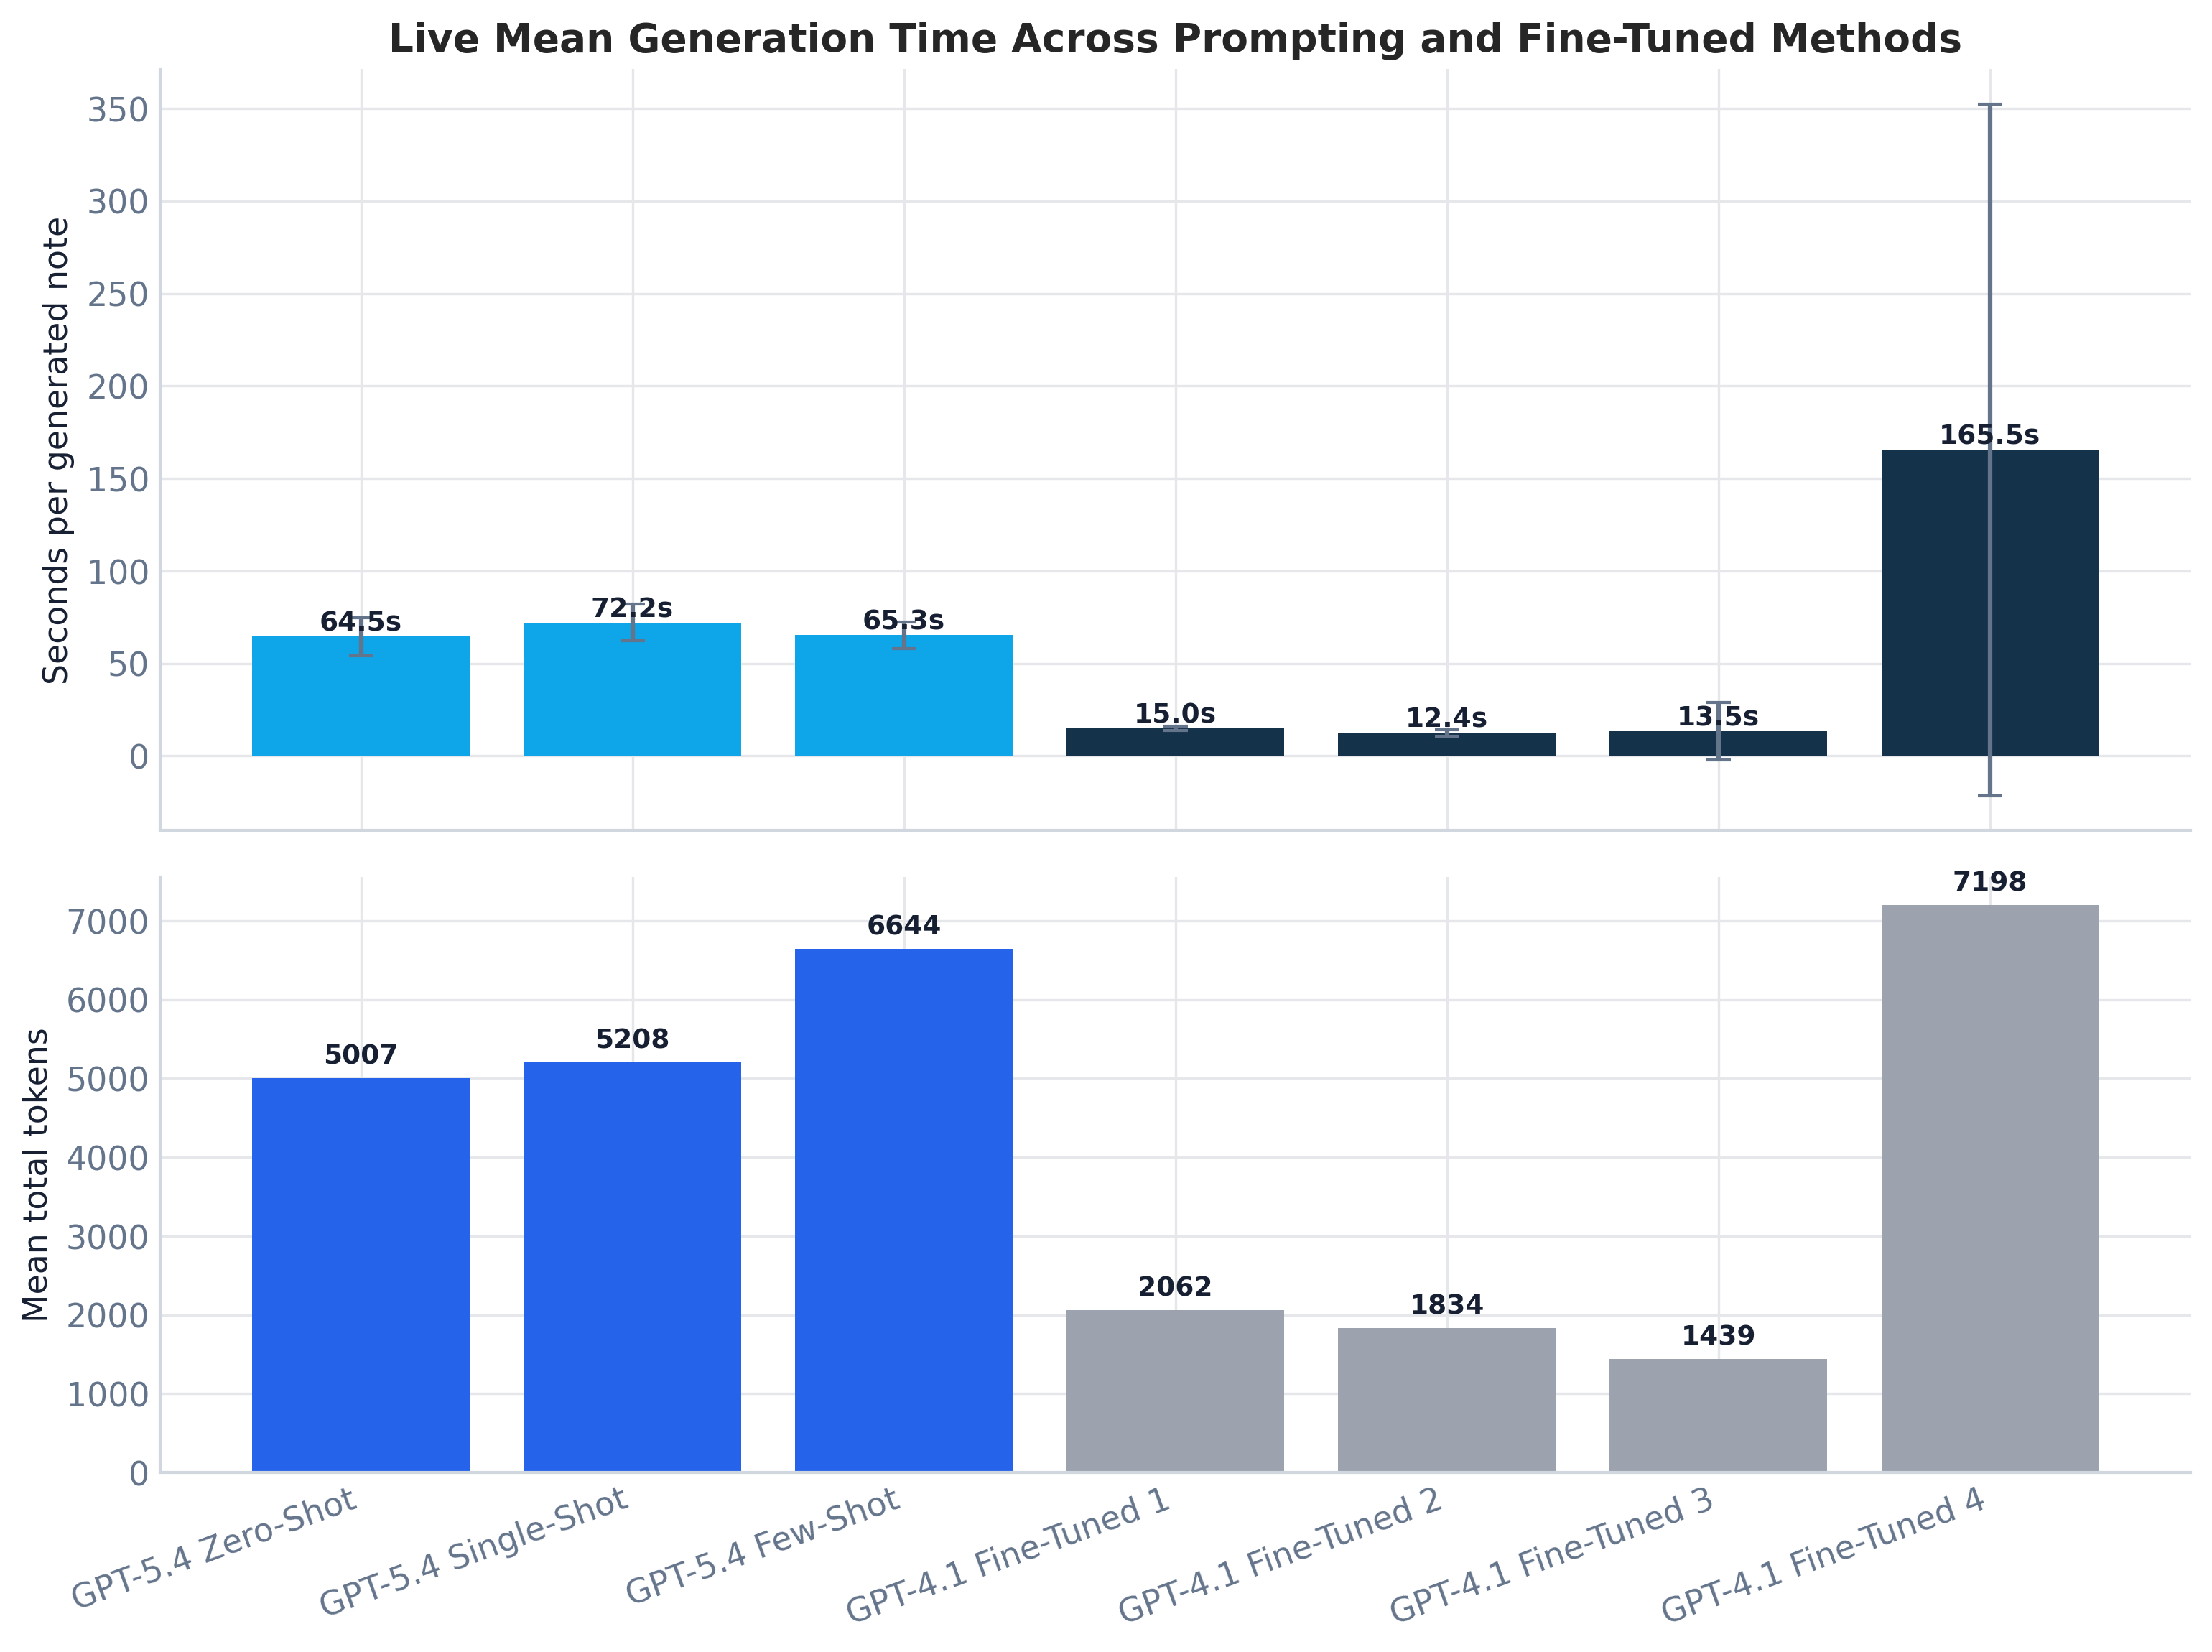
\includegraphics[width=0.9\textwidth]{figures/method_timing_comparison}
    \caption{Time to Produce a Result for All Seven Tested Methods}
    \label{fig:timing_all_methods}
\end{figure}

Figure \ref{fig:timing_all_methods} shows the timing profile across all seven tested methods. Among the prompt-engineering baselines, zero-shot averaged 64.5s, few-shot 65.3s, and single-shot 72.2s. The fastest stable fine-tuned deployments were GPT-4.1 Fine-Tuned 2 at 12.4s mean latency and GPT-4.1 Fine-Tuned 1 at 15.0s. GPT-4.1 Fine-Tuned 3 was faster on average than the prompt baselines, but that mean hides degenerate very short outputs in two cases and a much longer response in the third. GPT-4.1 Fine-Tuned 4 was the slowest and least stable overall, averaging 165.5s because one run expanded to 16,384 completion tokens and took 429.8s. The practical lesson is that fine-tuning can reduce latency dramatically, but only if the deployed checkpoint remains behaviourally well-controlled.

\begin{figure}[H]
    \centering
    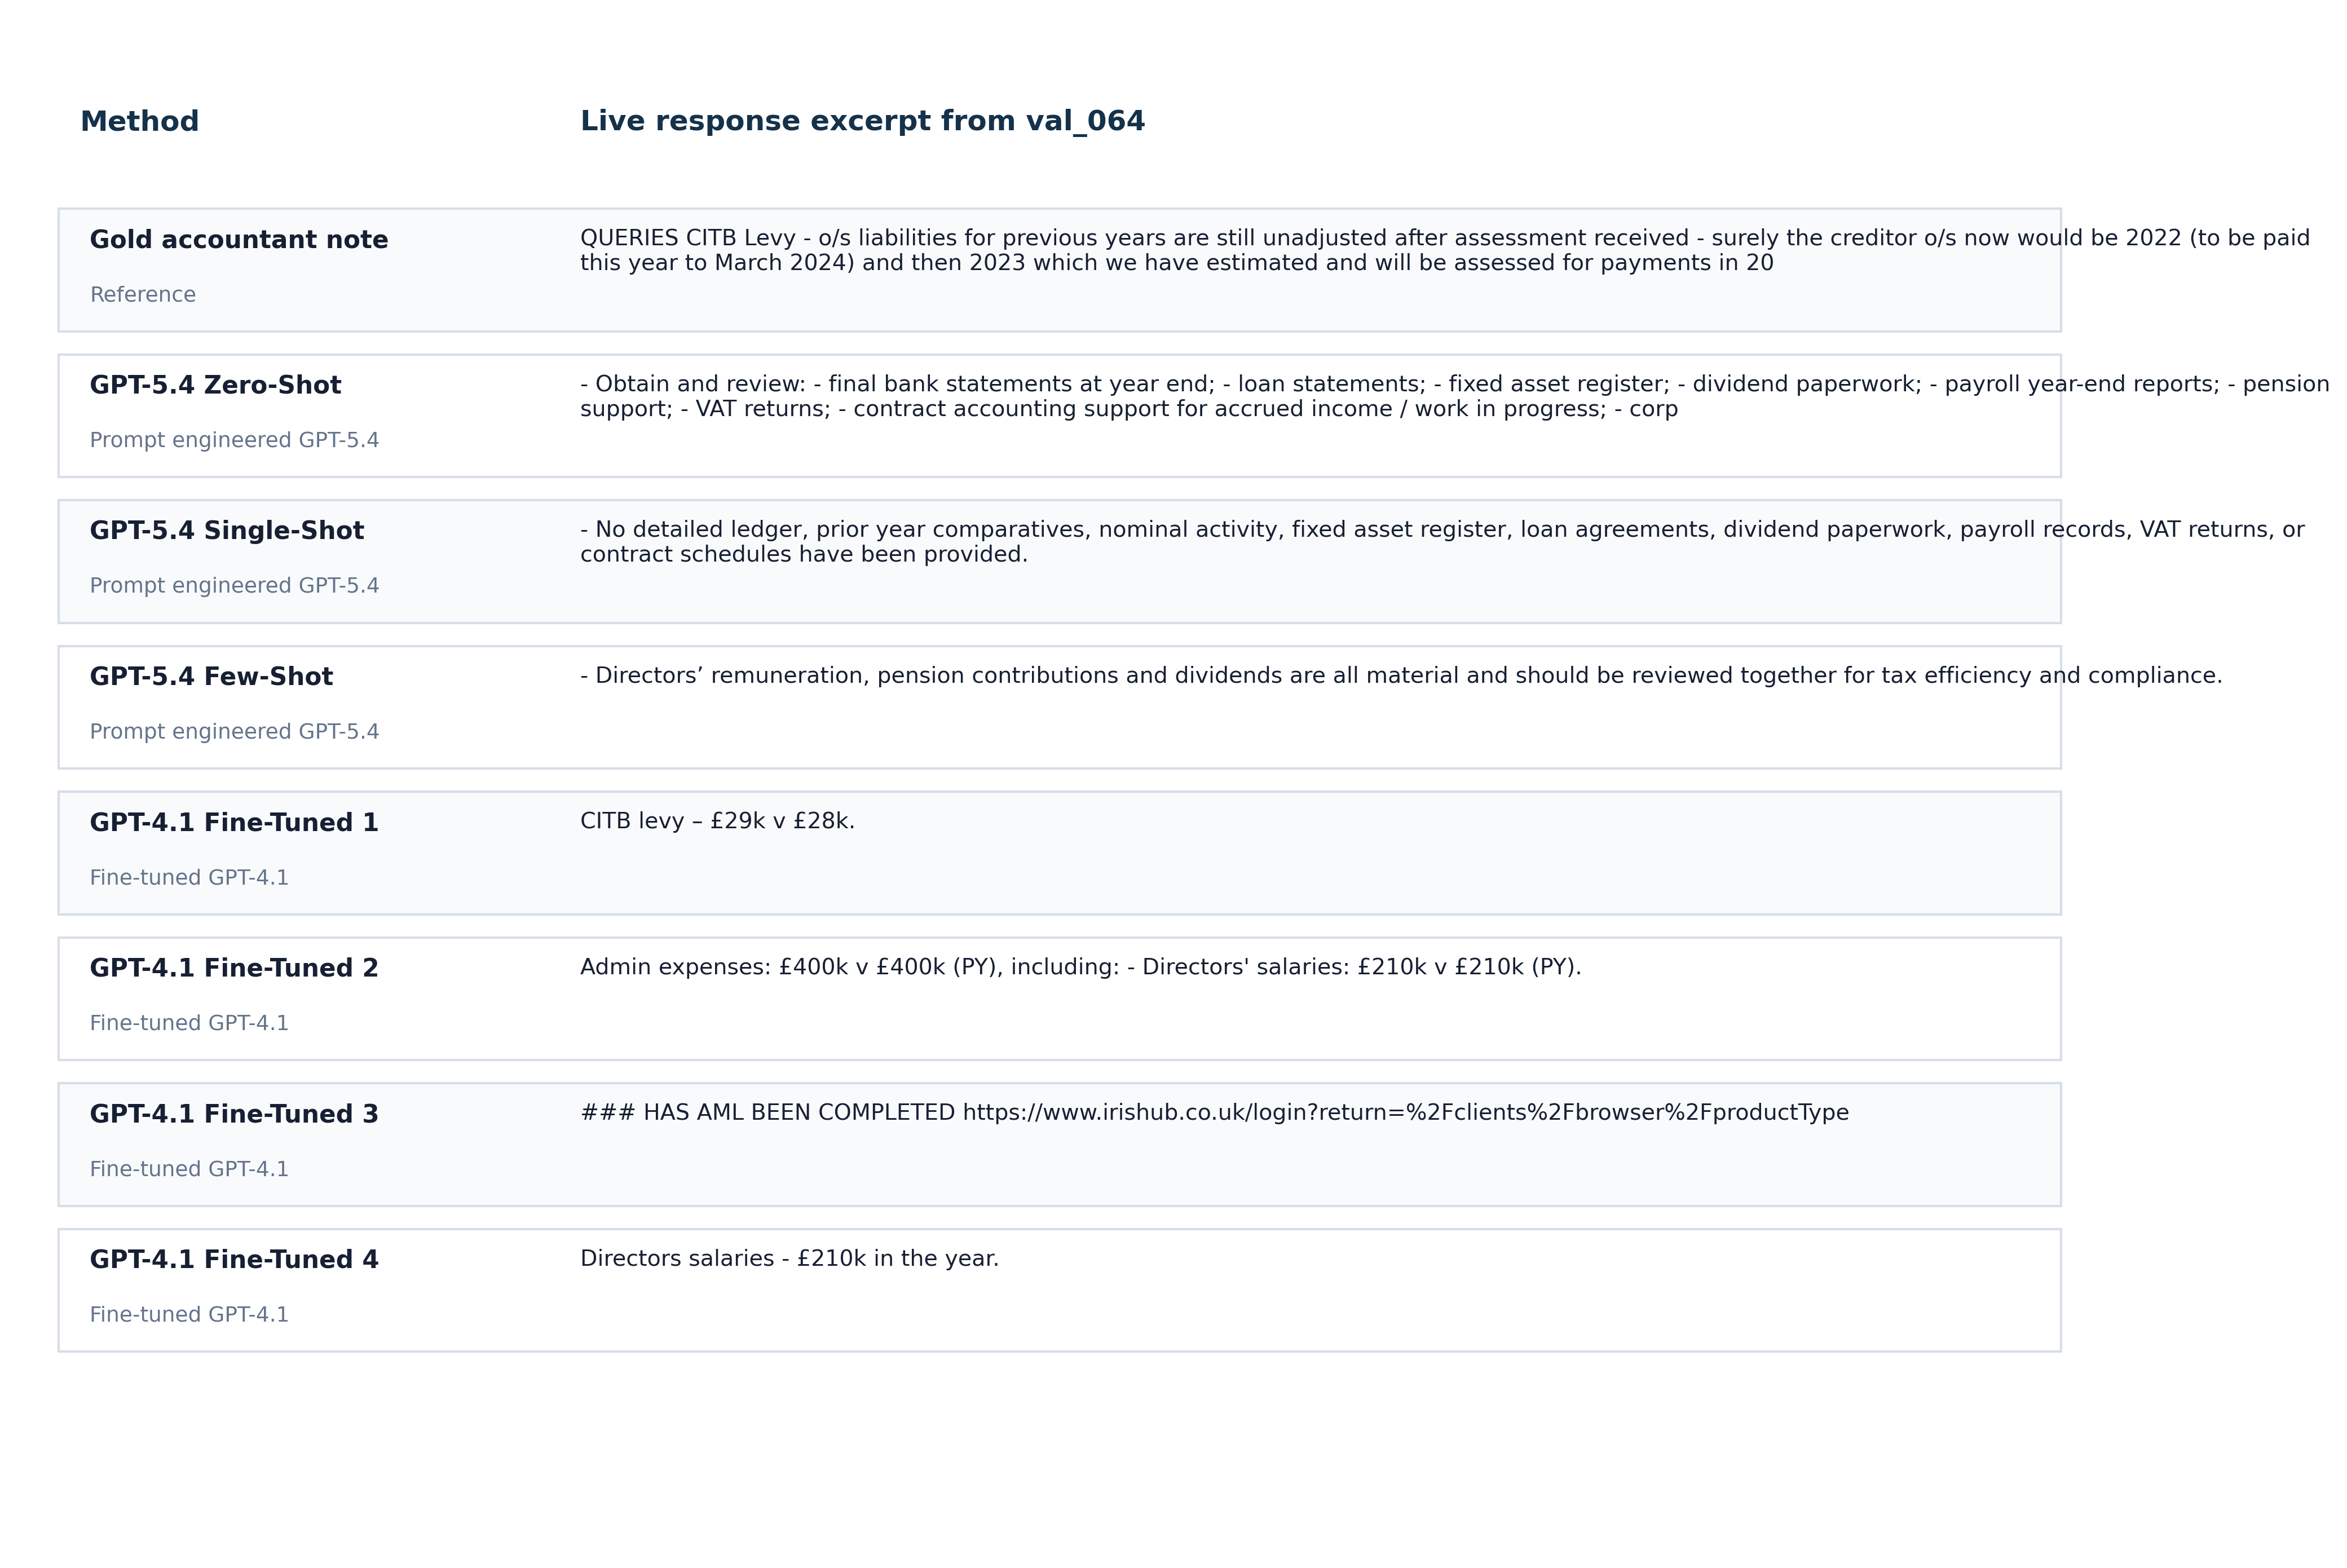
\includegraphics[width=\textwidth]{figures/method_output_comparison}
    \caption{Side-by-Side Comparison of Response Types on the CITB Liability Validation Case}
    \label{fig:method_output_comparison}
\end{figure}

The side-by-side comparison in Figure \ref{fig:method_output_comparison} makes the trade-off easier to see than a metric table alone. The gold accountant note raises a specific CITB levy adjustment query. The prompt-engineered GPT-5.4 outputs remain much broader and more generic, often asking for file-completion evidence rather than surfacing the liability issue directly. Fine-Tuned 1 and Fine-Tuned 2 are much faster and more numerically focused, but they still behave more like compressed management commentary than a targeted review note. Fine-Tuned 3 collapses to an AML stub on this case, while Fine-Tuned 4 does ask review-style questions but is less disciplined and, on another case in the subset, becomes extremely verbose. The figure is useful because it shows that fluent output and review-relevant output are not the same thing.

The share-issue case remained a useful stress test even though it is not the main comparison figure. On \texttt{val\_084}, several methods drifted away from the unresolved investment paperwork and instead produced broad profit-and-loss commentary. That failure mode matters in practice because a smooth narrative that drops the open equity query is less useful than a rougher note that keeps the review point visible.

\section{Human Evaluation Survey}
Two survey instruments were used to evaluate the practical value of the system. Survey 1 measured baseline manual effort and pain points before AI assistance. Survey 2 measured accountant perceptions of AI-generated notes after review. For the final evaluation framing used in this dissertation, the reviewed notes are treated as outputs from \textbf{GPT-4.1 Fine-Tuned 2}, which was selected as the human-evaluation candidate because it provided the best balance of stable output length, review-note structure, and latency in the live benchmark. The survey sample contained 10 professional respondents across accountants, client account managers, an audit supervisor, and partners.

\begin{figure}[H]
    \centering
    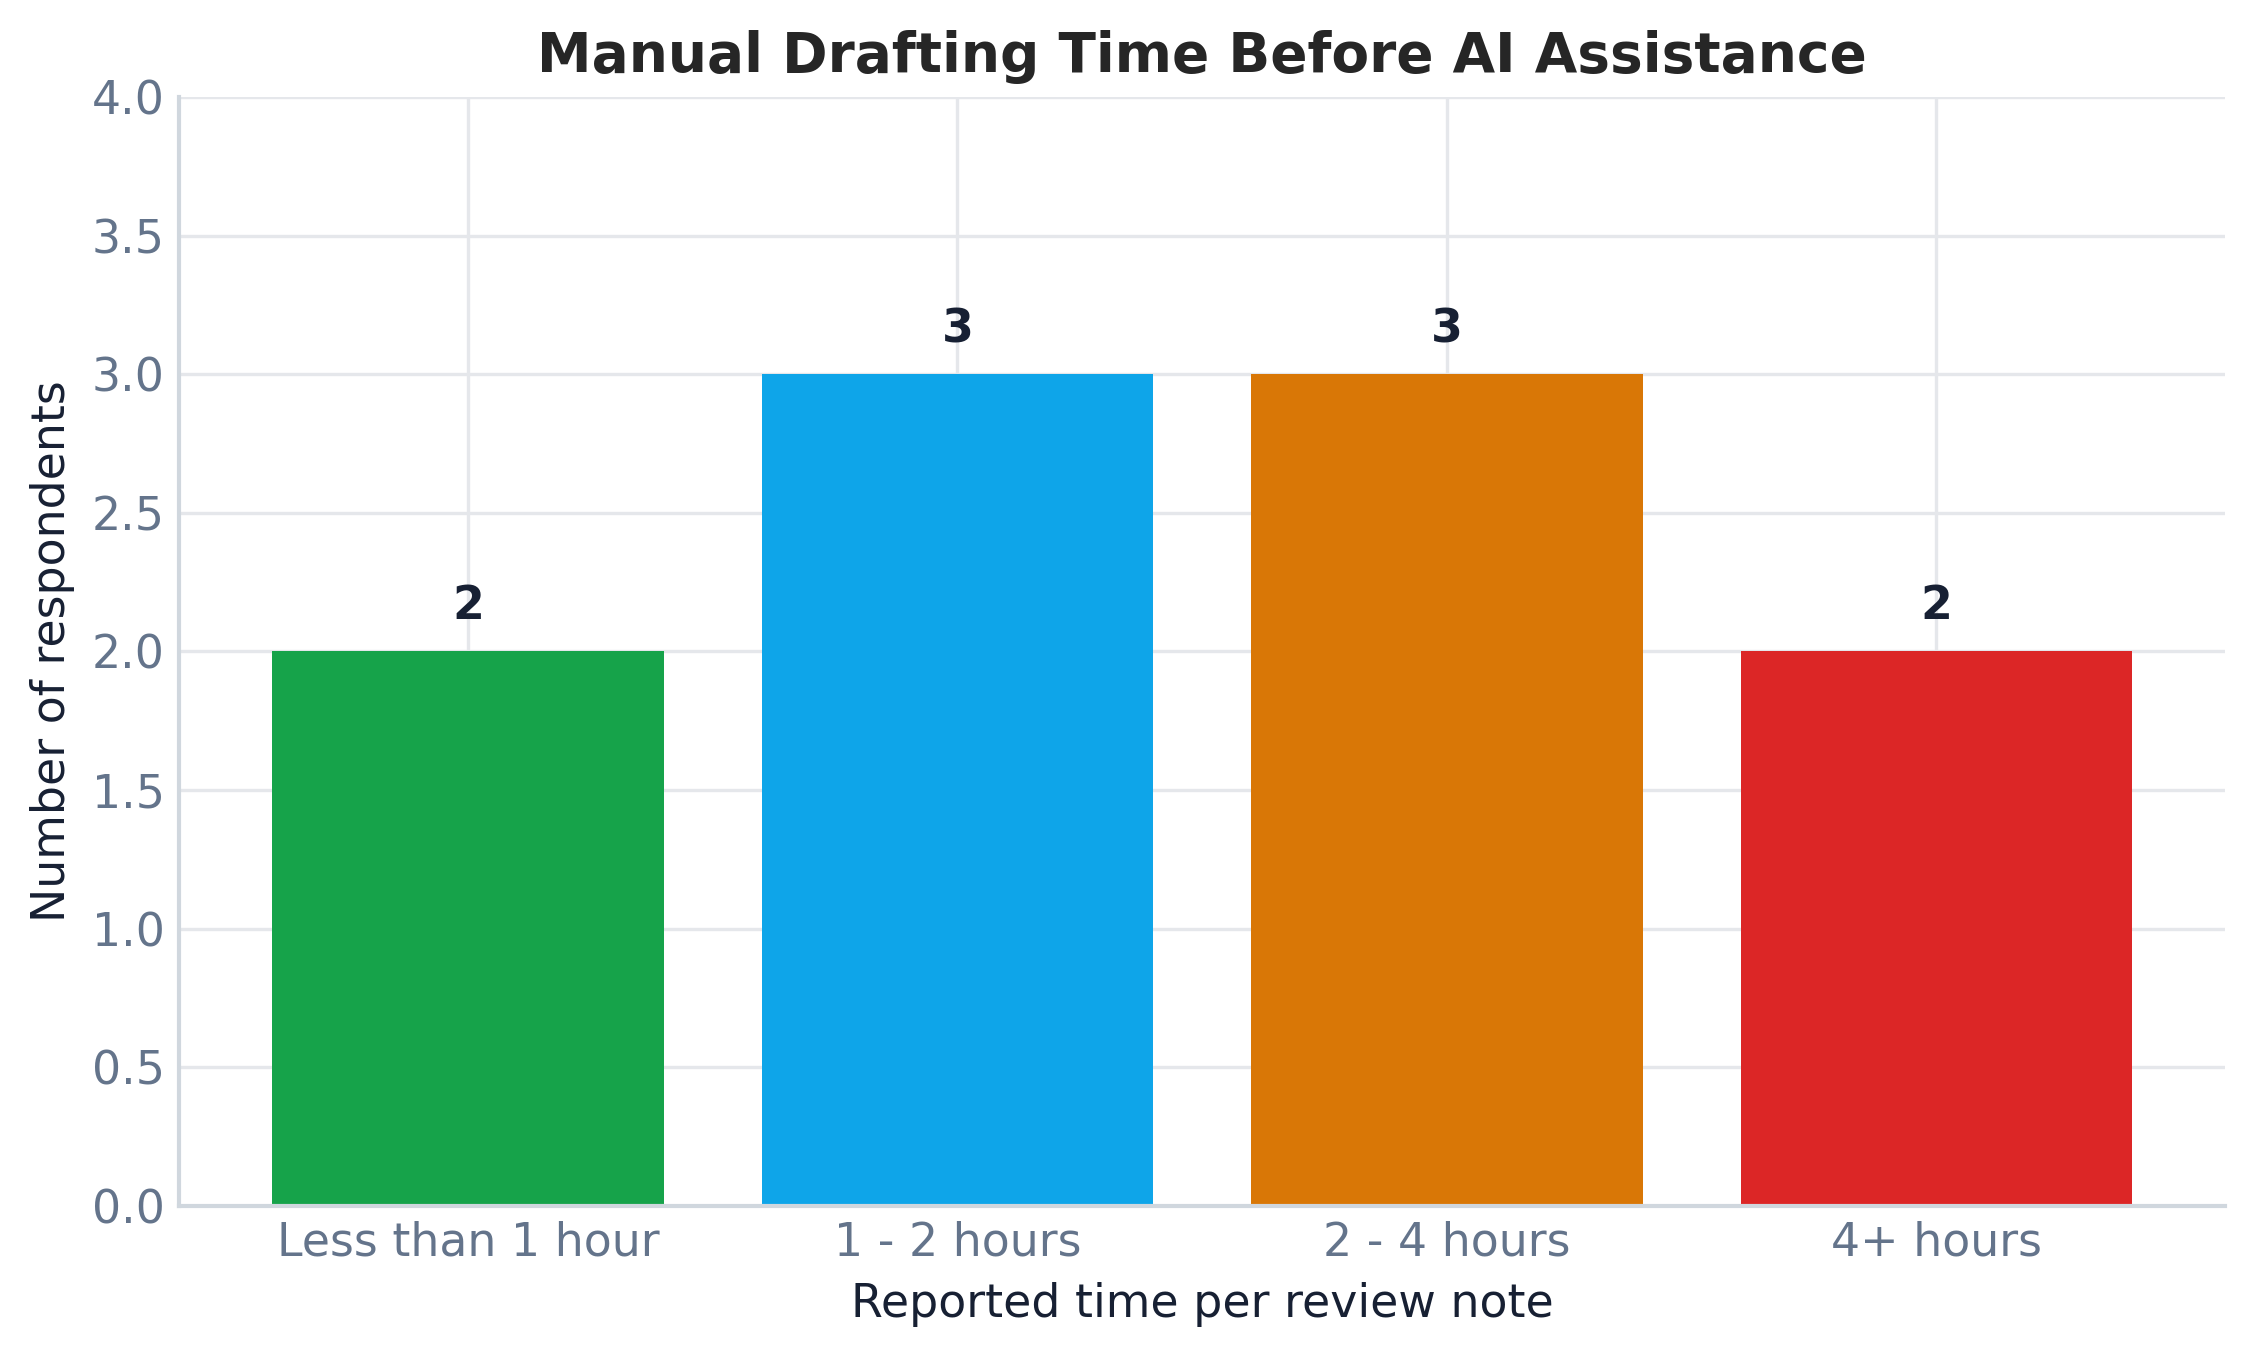
\includegraphics[width=0.78\textwidth]{figures/survey_manual_time}
    \caption{Manual Drafting Time Reported Before AI Assistance}
    \label{fig:survey_manual_time}
\end{figure}

The baseline survey demonstrates that manual review-note production remains time-consuming. Eight of the 10 respondents reported spending at least one hour per review note, and five reported spending two hours or more. The approximate midpoint average was 2.35 hours per note. The most difficult note categories were evenly distributed across Fixed Assets, Accruals and Prepayments, Directors' Remuneration / DLA, Related Party Transactions, and Debtors and Creditors, indicating that the system must handle a broad range of accounting judgement tasks rather than a single repetitive template.

\begin{figure}[H]
    \centering
    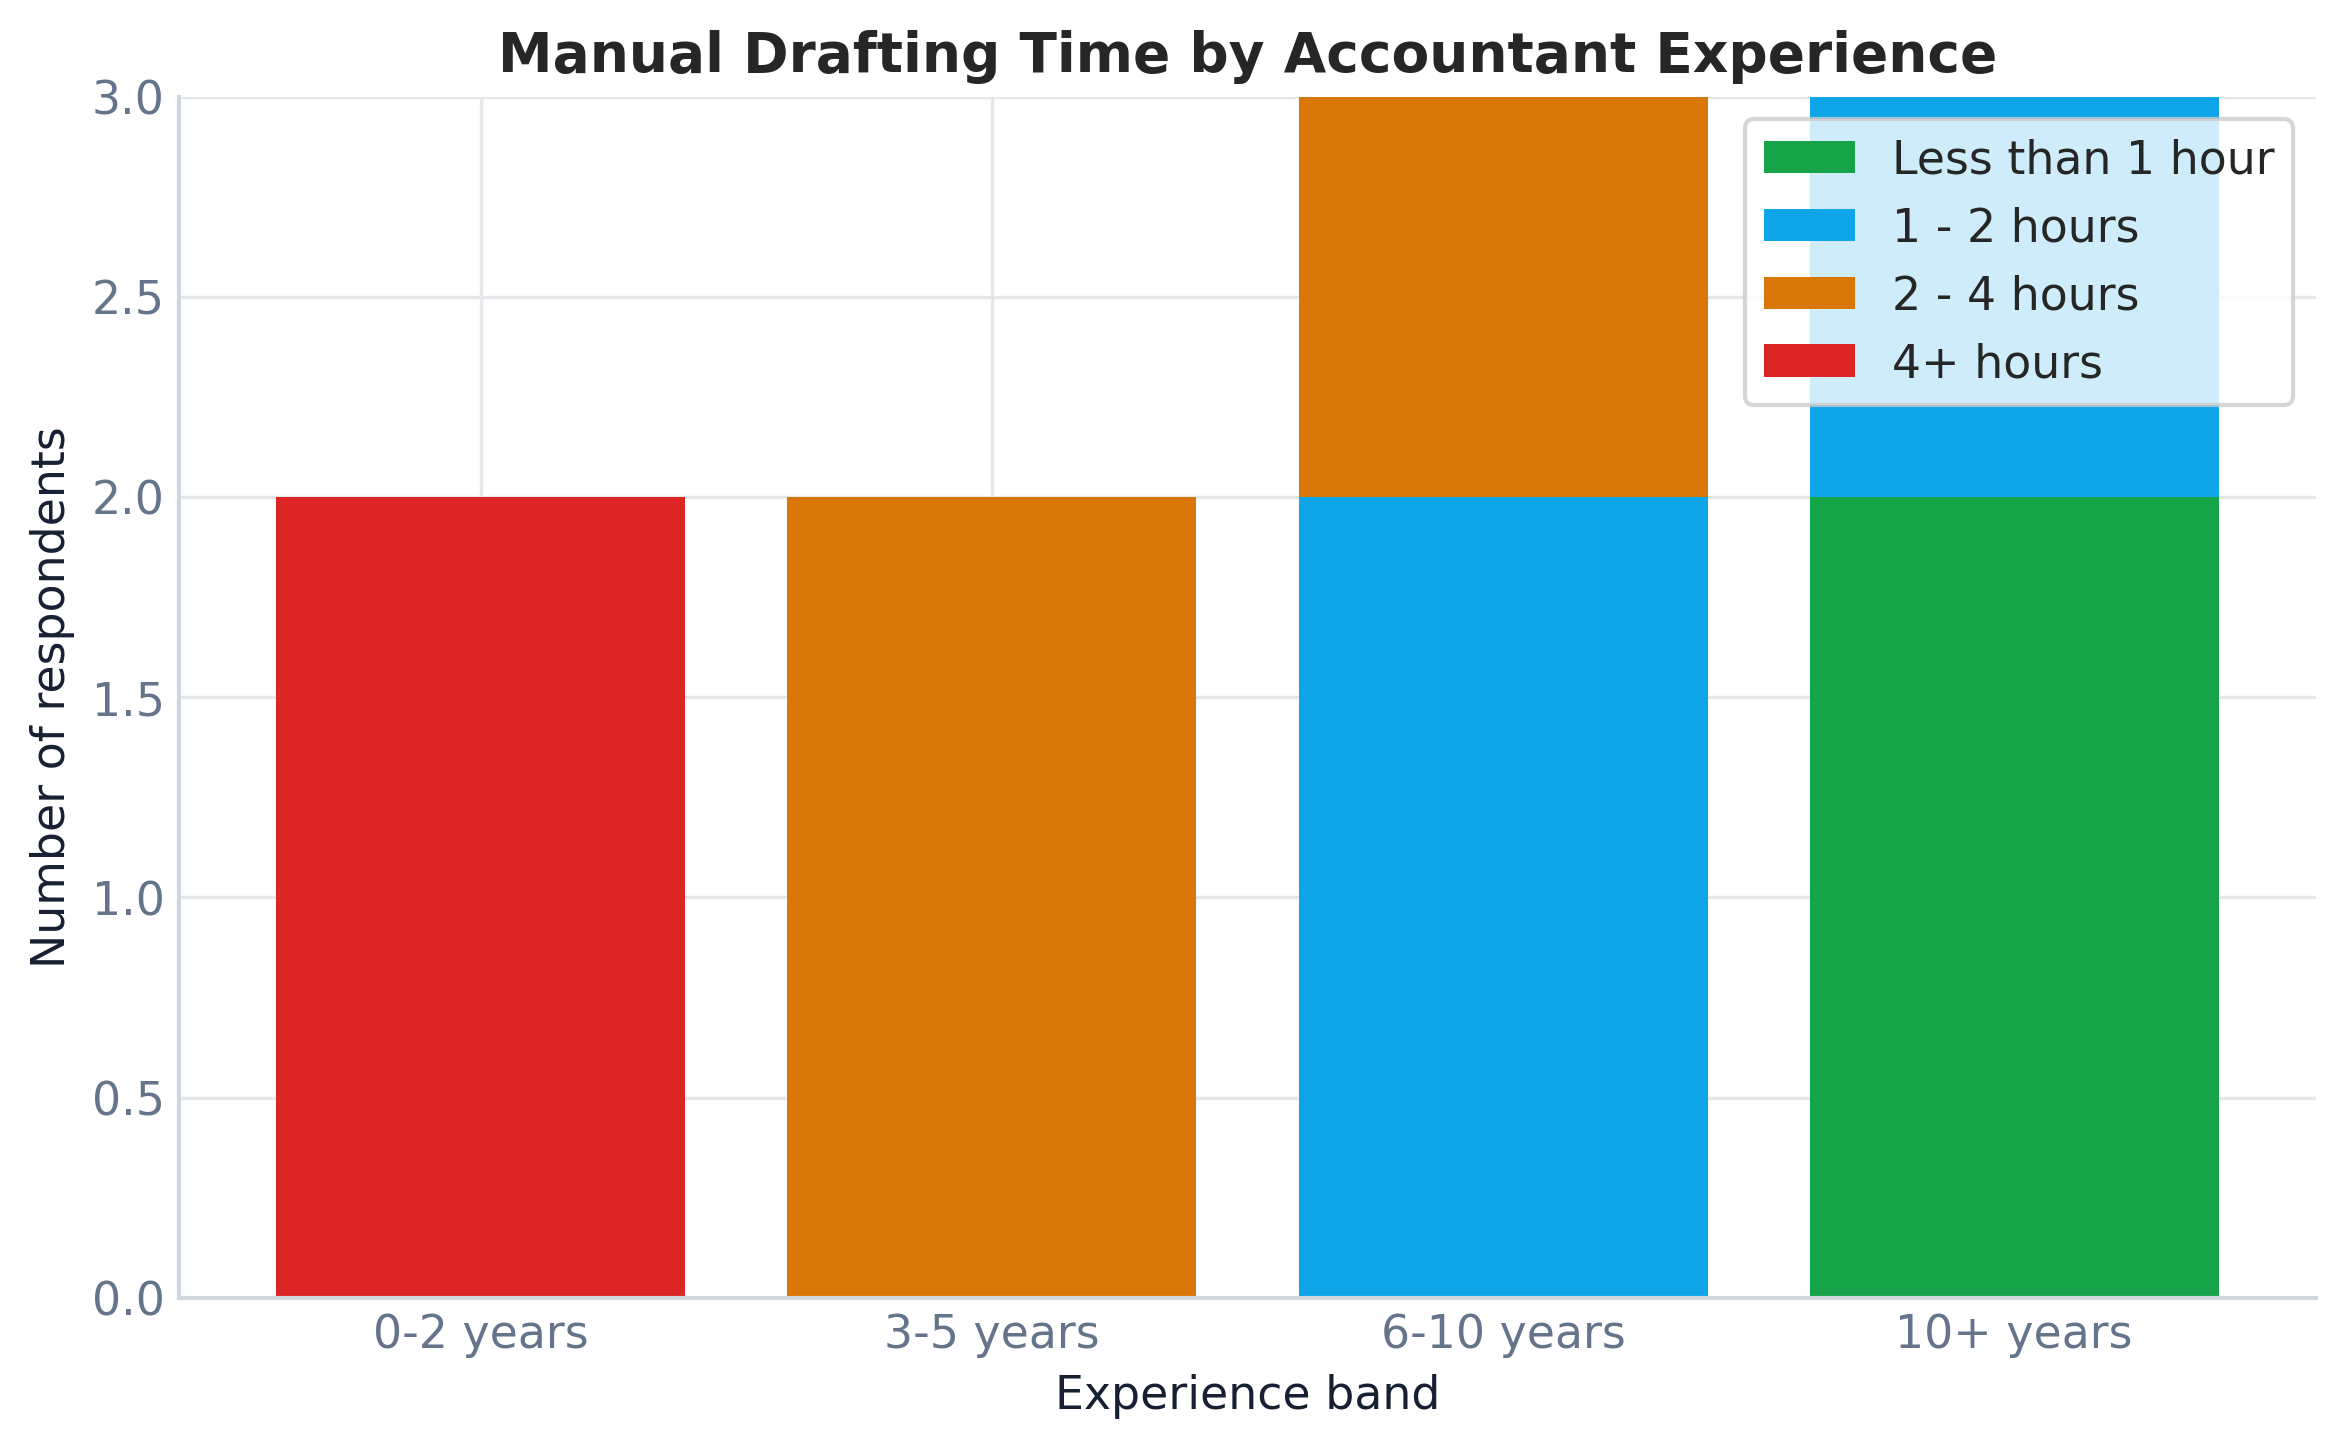
\includegraphics[width=0.82\textwidth]{figures/manual_time_by_experience}
    \caption{Manual Drafting Time by Experience Band}
    \label{fig:manual_time_by_experience}
\end{figure}

Figure \ref{fig:manual_time_by_experience} adds a little more detail to the baseline picture. The newer respondents cluster in the longer drafting-time bands, while the partner and senior-manager group is concentrated in the shorter bands. That pattern helps explain why the system was framed as a first-draft assistant rather than a replacement for judgement.

\begin{figure}[H]
    \centering
    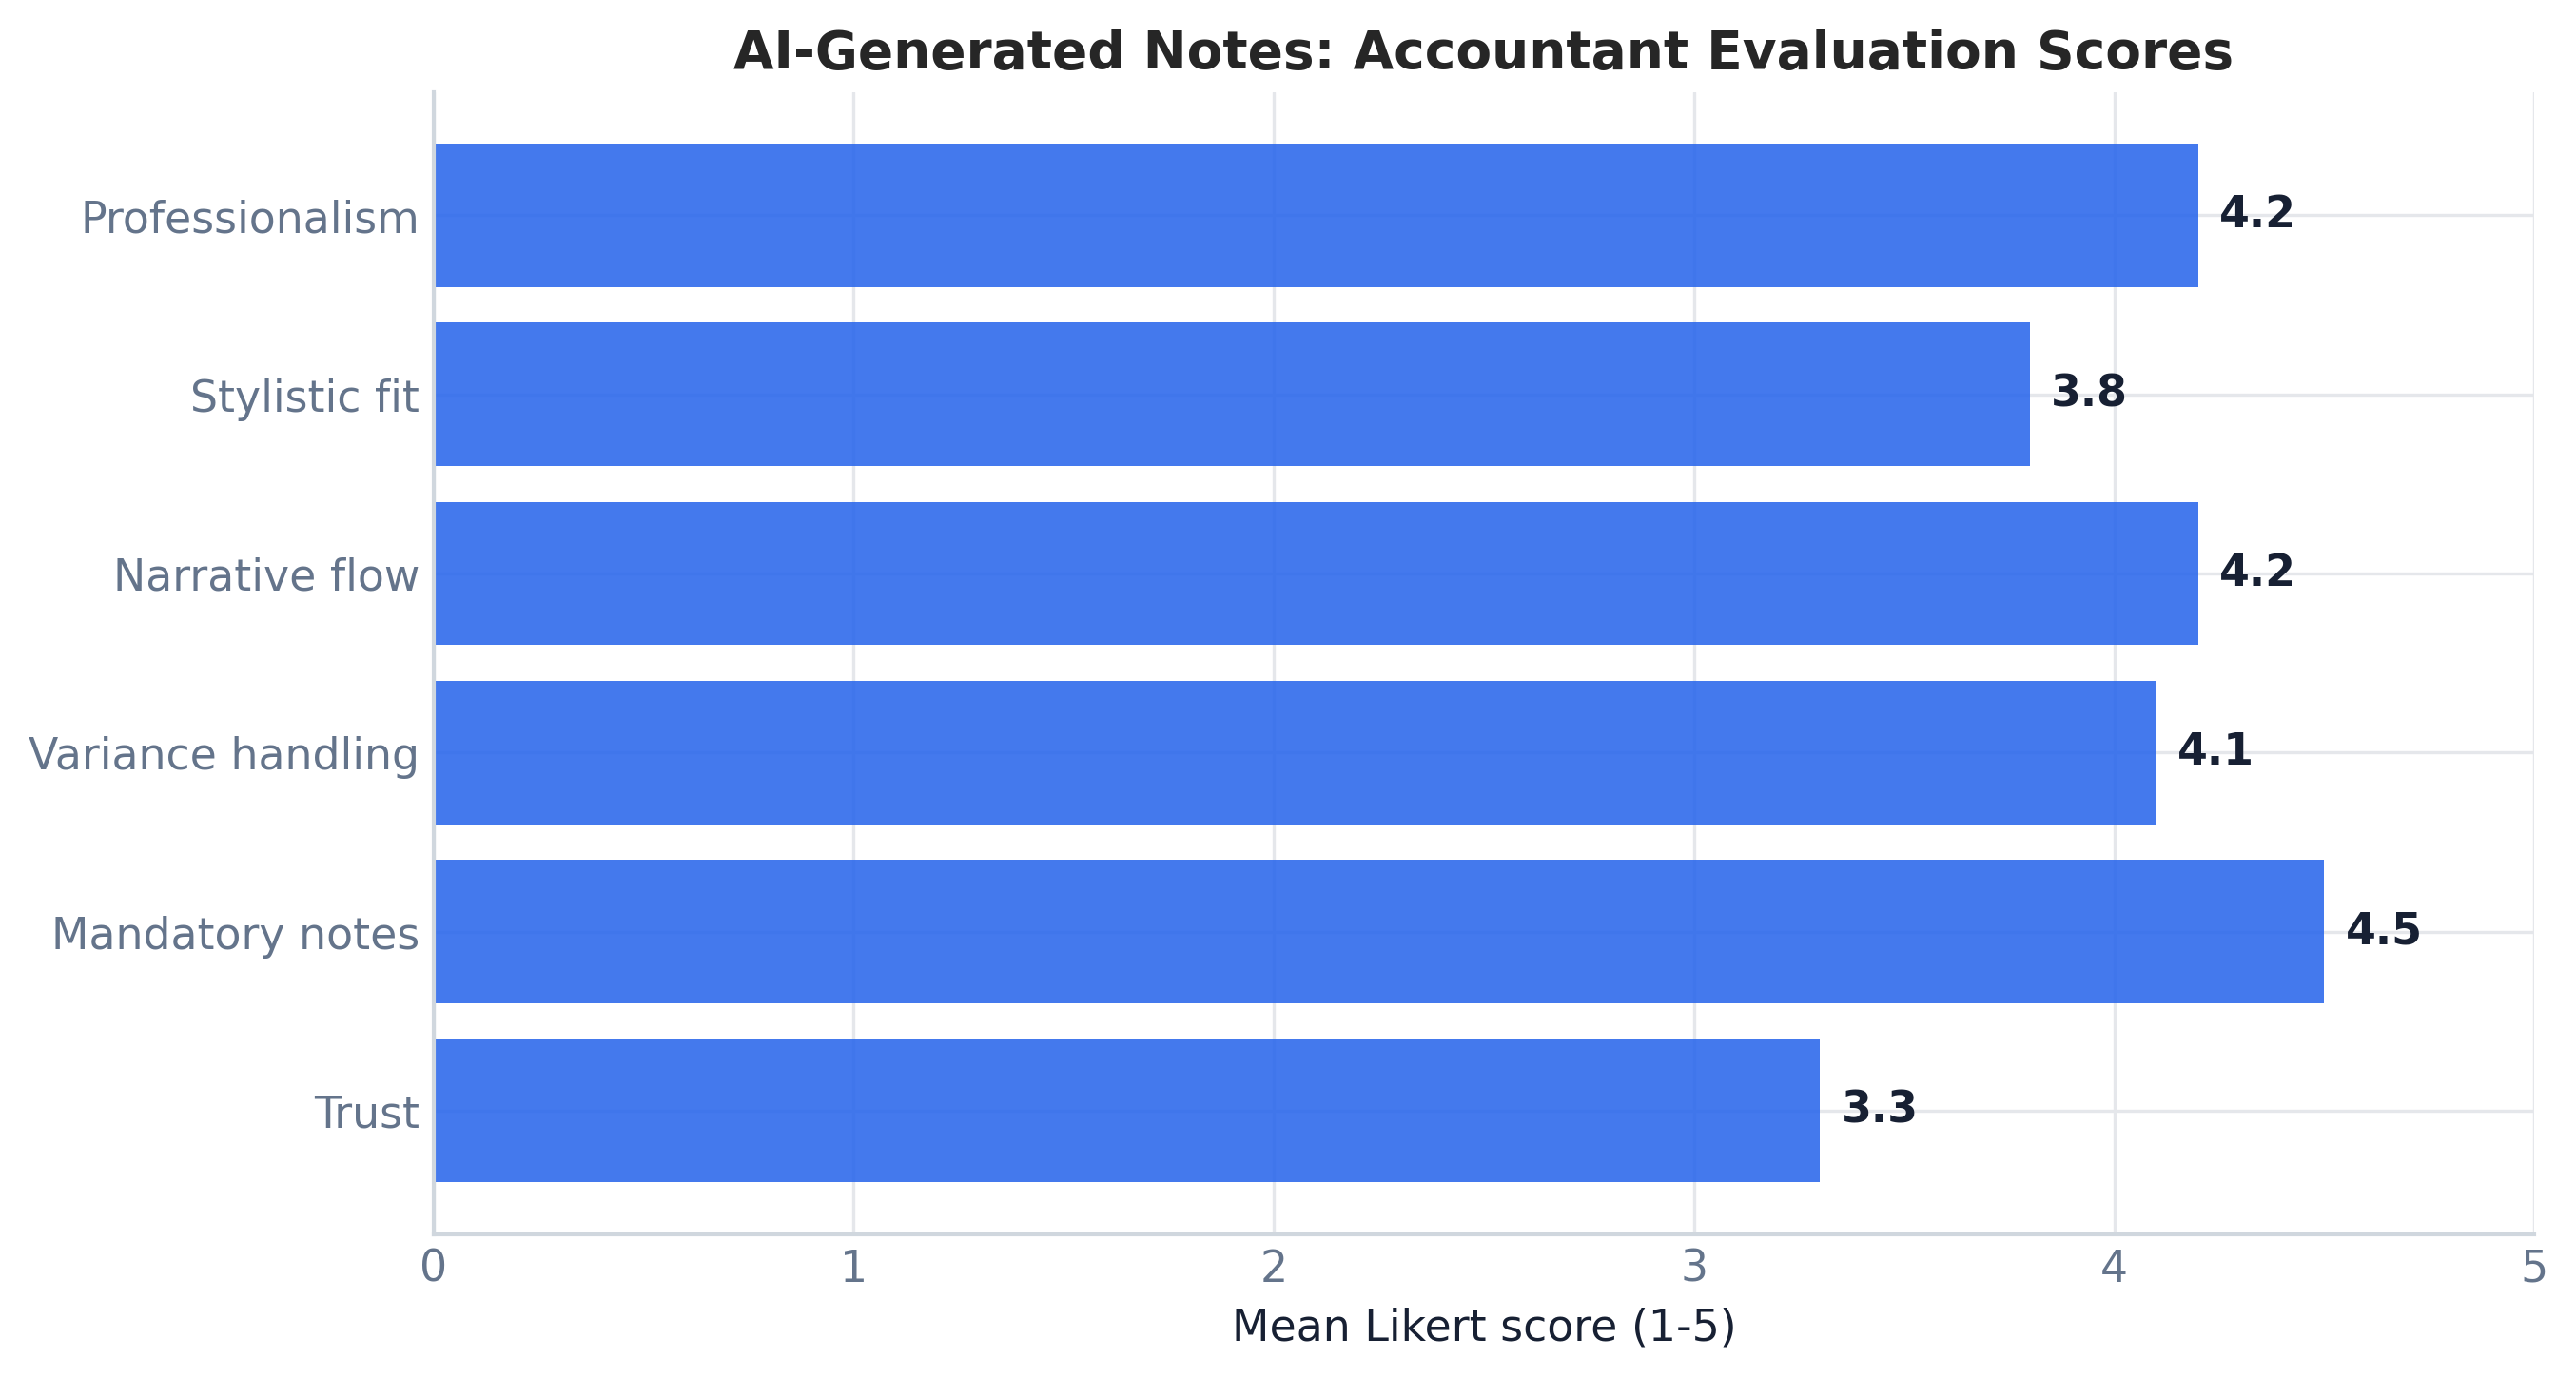
\includegraphics[width=0.82\textwidth]{figures/survey_ai_scores}
    \caption{Accountant Evaluation Scores for AI-Generated Notes}
    \label{fig:survey_ai_scores}
\end{figure}

Survey 2 shows positive but mixed professional reception. The AI notes achieved an overall mean score of 4.02 out of 5 across the six evaluation dimensions. Mandatory-note coverage was the highest-scoring category, with a mean of 4.5, followed by professionalism and narrative flow at 4.2. Trust received the lowest mean score at 3.3, which supports the continued use of human review and provenance controls.

\begin{figure}[H]
    \centering
    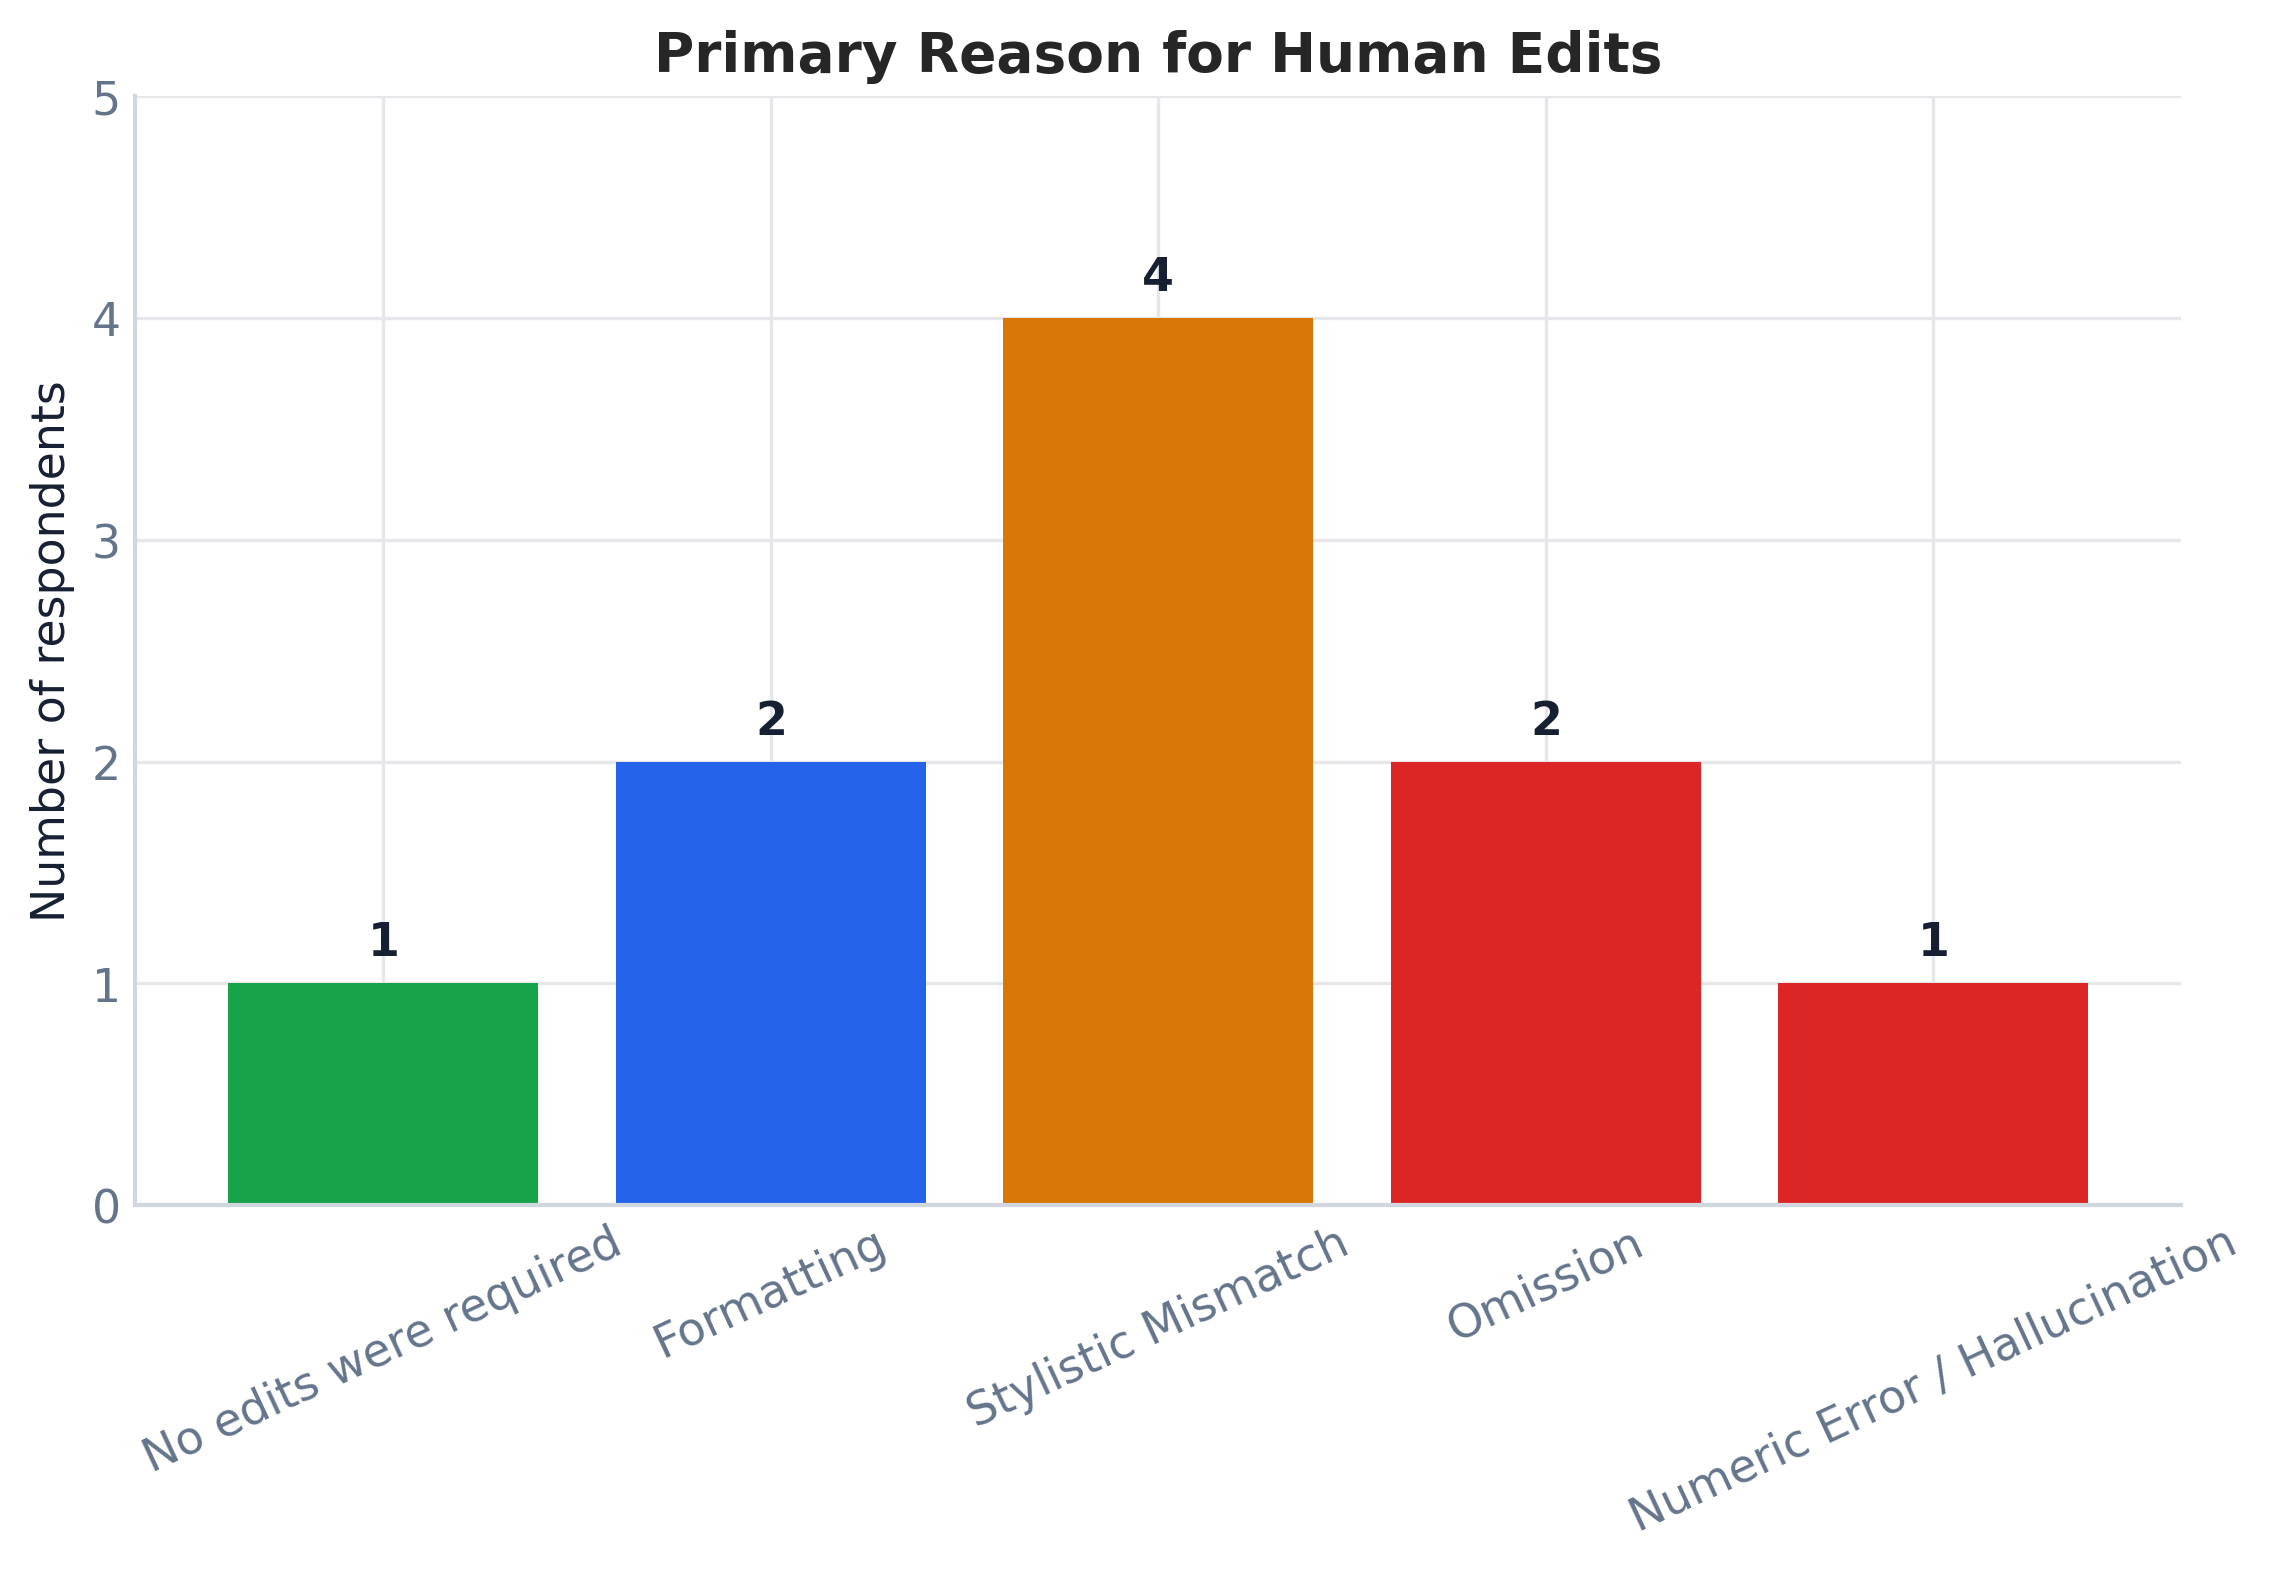
\includegraphics[width=0.78\textwidth]{figures/survey_edit_reasons}
    \caption{Primary Reason for Manual Edits After AI Generation}
    \label{fig:survey_edit_reasons}
\end{figure}

The edit-reason data is useful because it shows where the system still creates work for the reviewer. Stylistic mismatch was the most common reason for human editing, reported by four respondents. Formatting and omission were each reported by two respondents, while one respondent reported no required edits and one identified a numeric error or hallucination. This pattern suggests that the main remaining challenge is consistent alignment with firm-specific wording preferences.

The real examples help explain this result. A note about GDPR-related compliance spend may be factually correct yet still feel wrong to an accountant if it does not match the firm's expected phrasing or sequence of explanation. A director-loan note may contain the correct amounts but still require editing if it presents a tax-sensitive issue too casually. Professional acceptability in accounting writing depends on tone, order, and caution as well as factual extraction.

\section{Research Risk Assessment}
The testing strategy directly addresses the main technical and ethical risks identified earlier in the dissertation:
\begin{itemize}
    \item \textbf{Data Privacy:} Production credentials are supplied through environment variables, sensitive client data is handled through Azure and Xero authenticated channels, and the dissertation workflow assumes minimisation, pseudonymisation, and retention limits before any prompt leaves the firm's boundary.
    \item \textbf{Hallucination:} The LLM is constrained by deterministic trial balance and transaction context, then evaluated against accountant-authored validation targets.
    \item \textbf{Over-Reliance:} Survey trust scores show that professional review remains necessary; therefore, the system is framed as a first-draft generator rather than an autonomous signing tool.
    \item \textbf{Reproducibility:} The validation corpus, survey files, graph-generation script, live benchmark harness, and stored benchmark CSV provide a repeatable workflow for extending or re-running the results.
\end{itemize}

From a governance perspective, the main GDPR concern is not simply where the model runs, but whether the surrounding process remains proportionate. The evaluation assumes a narrow lawful purpose, accountant-only access, deletion of temporary exports after use, and a clear boundary between generated drafts and final signed workpapers. This matters most for narratives involving directors' loan accounts, payroll, legal disputes, or share issuances, where routine accounting notes can still contain personal or commercially sensitive data.
